\documentclass[11pt]{article}
\usepackage{enumerate}
\usepackage{amsfonts}
\usepackage{graphicx}
\pagestyle{empty} \setlength{\parindent}{0mm}
\addtolength{\topmargin}{-0.5in} \setlength{\textheight}{9in}
\addtolength{\textwidth}{1.75in} \addtolength{\oddsidemargin}{-0.9in}
\date{\today}
\begin{document}
\textbf{CS474 Bioinformatics \hfill \today\ \\
\\
James Bucher \\
Tyler Land \\
Kyle Mears \\
Christina Guiterrez \\
Ali Hajy}

\begin{center}
\textbf{Introduction}
\end{center}
While methods have been developed for detecting covarying amino acid regions in a single protein that interact together, little progress has been made to detect coevolution between two different proteins using covarying amino acids.  We develop a scoring algorithm that analyzes the amino acid sequences of two proteins, considers how conserved the regions of one protein are with respect to another protein, and attempts to quantify the amount of coevolution between the two proteins. \\

We begin with sequences of candidate protein pairs.  For a pair of proteins A and B, we search for a collection of homologs to each of those proteins and align all of the proteins.  We form the cross product of mutations across collection A with mutations across collection B and only consider pairs of mutations that belong to the same species.  Each pair of mutations is scored and that score is used to score the pair of proteins those mutations belong to.  A protein pair's score should be directly proportional to that pair's interrelatedness; a high score indicating that two proteins have evolved together.

\begin{center}
\textbf{Data (search.py and search\_blast.py)}
\end{center}
Since we are trying to find interactions between proteins our input is
of course a set of proteins that we want to find the interactions
between. These are supplied as a series of fasta files which are then
used to search blast. \\

This blast search is done using the {\bf NCBIWWW.qblast} supplied by
Biopython. The search results are then stored in a temporary xml file
for testing purposes (to reduce stress on the blast server). The
results from blast are read and then written to a temporary file
since the Biopython {\bf NCBIXML} module will only accept a file
handle as input. This gives us a set of records that can be turned
into useful homologs. When iterating through the records a
dictionary representing each homolog of the following form is
created: \\
{\footnotesize
\begin{verbatim}
{'searchQuery': <the function argument searchQuery>,
 'proteinName': <the function argument proteinName>,
 'species':{ 'species-1': [{'id':'species-1', 'seq':<protein-seq-1>, 'desc':<blast-desc-1>, 'uid': 1},
                           {'id':'species-1', 'seq':<protein-seq-2>, 'desc':<blast-desc-2>, 'uid': 2},
                          ],
             'species-2': [{'id':'species-2', 'seq':<protein-seq-3>, 'desc':<blast-desc-3>, 'uid': 3}
                          ],
             . . .
           }
}
\end{verbatim}
}
This approach makes it easy to export data to standard out via
JSON. This allows us to use multiple scripts we have written to
be used much like the Unix command line tools; chaining them
together as pipelines. When choosing candidate protein homologs
an E-Value (from the blast results) of $1.0 \times 10^{-5}$ is used
since this is the current standard for homologs from blast. Furthermore, if
there is more than one protein returned for a species then the first
is chosen abitrarily. This is known as a paralogue and is caused by
gene duplication in an organism where one copy of the gene starts
specializing for one function and the other continues performing the
same old function. This is hard to distinguish if the divergence of
the gene is recent (since the sequences will be almost identical). As
such it is currently outside of the scope of this project to deal with
this. However, the current layout of the software allows for the
possibility of multiple paralogues to be included in a collection of
homologs so that if this issue needs to be addressed in the future it
will be possible to do so. \\

After homologs are acquired from BLAST they need to be aligned. For
this we use ClustalOmega since it can be used via standard in and
standard out to align sequences. A subprocess is then opened to
communicate with ClustalOmega and the results are then parsed to get
the resulting alignments and the homolog structure above is updated
with the sequences that are now aligned. \\

The resulting series of homologs (for each input file) are turned
into a list and then written to standard out as a JSON string. \\

All of the above is wrapped up into the script "search\_blast.py"
which depends on the file "search.py" to do the actual searching. \\

\begin{center}
\textbf{Methods}
\end{center}
After searching BLAST for homologs and preprocessing the data it is
then fed into a script that creates pairs of homologs
(map.py). Given a set of homologs map.py creates pairs of homologs
between all elements of the set supplied which is then given to
reduce.py as input. reduce.py then takes these pairs and runs an analysis for every pair
of proteins. \\

Analysis starts with finding the unique mutations in each column of
the alignment of the set of homologs. Columns are currently filtered out by
the following criteria: \\

\begin{itemize}
  \item If the column contains a gap in at least one protein then it
    is filtered out.
  \item If: 
    \begin{center}
      $\frac{\mbox{number of types of amino acids in column}}{\mbox{total number
          of amino acids in column}} > \mbox{MAX\_VARIATION\_RATIO}$
    \end{center}
    Then the column will be filtered out since it has too much
    variation and is likely a non-conserved region of the protein.
  \item If there are no mutations in the column then it is filtered out.
\end{itemize}

This results in a data structure that only contains mutations that are
conserved enough for analysis (a series of columns each of which
contains at least one mutation). Furthermore a mapping between the
original amino acid position and the new position is kept so that this
information is not lost. \\

The next step of analysis produces a set of points that are possible
concurrent mutations between the proteins. In order to do this we take
the Cartesian product of the mutations but only between the same
species. This process produces a set of coordinates where the $x$
coordinate corresponds to the position in homolog set $A$ and the $y$
coordinate is the position in homologue set $B$. These coordinates can be
repeated if the same combination of mutations occurs within two
species within the homolog sets. When producing these coordinates a
coordinate is only produced if the species name for a mutation
corresponds. Otherwise the mutation is not within the same species and
therefore cannot be a coevolution site.\\

Along with the coordinate several other pieces of information are
calculated. First a BLOSUM matrix is used for each of the position to
calculate the BLOSUM score for each mutation (a higher score is more
conserved). When calculating this score it is assumed that the amino
acid changed from the most common amino acid to the current amino acid
when looking up the score in the matrix. That is to say if the column
included 12 instances of 'T' and one instance of 'A' and one instance
of 'D' then the program would assume that both 'A' and 'D' changed
from 'T'. If there is a tie then the choice is made abitrarily
(although the column filter is designed to catch these kind of cases
so that they don't influence the results). \\

Then the BLOSUM score is modified with a score penalty of the
following:
\begin{center}
  $1 - \frac{\mbox{number of amino acids across homologs in mutation}}{\mbox{VARIATION\_AMINO\_ACID\_SCORE\_PENALTY}}$
\end{center}
This adjusts the scores for columns that have more variation to be
lower (corresponding to less conserved). The
VARIATION\_AMINO\_ACID\_SCORE\_PENALTY variable can be used to adjust
how much variation is penalized. \\

After calculating and adjusting the BLOSUM score for each mutation the
mutations in the coordinate are given a distance based score under the
assumption that a large mutation in one amino acid in protein A will
correspond to a large mutation in an amino acid in protein B. This is
calculated using the following formula. \\
\begin{center}
  $\mbox{DIST\_SCORE} = $
  $\frac{1.0}{(1.0 + |\mbox{BLOSUM\_SCORE\_A} - \mbox{BLOSUM\_SCORE\_B}|)}$
\end{center}
In this case the score will be higher when the BLOSUM scores are
closer so that mutations that would cancel each other out will receive
higher scores. \\

The above scores and the coordinates within each protein are then
turned into a tuple that is then put through a post filtration to
remove more erroneous results and after this filtration total scores
are calculated. \\

This filtration is preformed by the following process:
\begin{enumerate}
  \item If the DIST\_SCORE is below the
    DELTA\_MUTATION\_SCORE\_MINIMUM then discard the tuple.
  \item If the combined BLOSUM score from both proteins A and B is
    between MAX\_ADD\_MATRIX\_SCORE and MIN\_ADD\_MATRIX\_SCORE then
    the tuple is discarded. This is to prevent non-extreme changes
    from entering results.
\end{enumerate}

After the filtration the DIST\_SCORE is summed over all tuples that
were left after filtration in order to get an overall score for the
protein pair. Then this raw score is normalized by the following equation: \\

$\mbox{FINAL\_SCORE} = $ \\
\begin{center}
  $\frac{\mbox{SUM\_OF\_TUPLES} \times
    100000}{MIN(\mbox{SIZE\_OF\_PROTEIN\_A, SIZE\_OF\_PROTEIN\_B})^2
    \times \mbox{COMMON\_SPECIES\_COUNT}}$
\end{center}

These results are then printed out on one line along with the protein
names and other relevant information in a comma separated value format
for ease of use with a spreadsheet program. \\

Since these calculations have started taking a nontrivial amount of
time for even 14 sample proteins (since the number of combinations is
on the order of $N^2$ where $N$ is the number of input proteins) the
programs are setup to run on Hadoop using the "run-hadoop.sh"
script. When run on Hadoop a sizeable speedup should be achieved
since the calculations are CPU bound. However given the
amount of time that Hadoop jobs take to start this would only make
sense for jobs that include a large number of proteins to be compared.

\begin{center}
\textbf{Result}
\end{center}

Previous researchers have tried to use amino acid covariance to predict binding between proteins, with little success.  
Below is an example of results from one of the first protein interaction predictors using amino acid covariance.

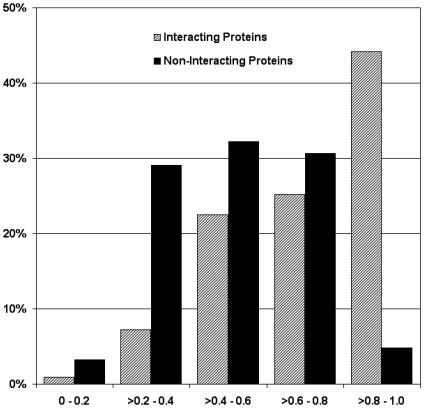
\includegraphics[width=4.25in,height=4.25in]{hi.png}
Score out-put of program vs percent of protein pairs within that score range (Tan SH, Zhang Z, Ng SK. ADVICE:\emph{automated detection and validation of interaction by co-evolution. Nucleic Acids Res 2004};32:W69-W72.)\\


Similar to previous results, ours do not give clear results and cannot be used to accurately predict binding using the output score.  This can be seen in table 1, where the score given to the interacting proteins are not discernibly different than the scores of non-interacting protein pairs.  \\

Table 1. Output scores of our program for interacting vs non-interacting protein pairs.  Six interacting pairs were tested and dozens of non-interacting pairs were tested.\\


\begin{center}
\begin{tabular}{ | l | l | p{5cm} |}
\hline
 & Interacting & Not Interacting \\ \hline
Mean & 19.8 & 20.6 \\ \hline
Median & 5.4   & 5.3  
 \\ \hline
Max & 76.7 & 278.7
 \\ \hline
Min & 2.1 & 0
 \\
\hline
\end{tabular}
\end{center}

Our program may be useful in determining binding sites of proteins known to interact.  For the known interacting proteins Rock1 and Rhoa, Graph 1 shows the amino acid positions at which our program predicts co-evolution.  Looking at Rhoa, more than half of the co-varying sites are located at or near the interaction site between the two proteins.  Using this data with the predicted structures for proteins could enhance the prediction of binding sites.\\

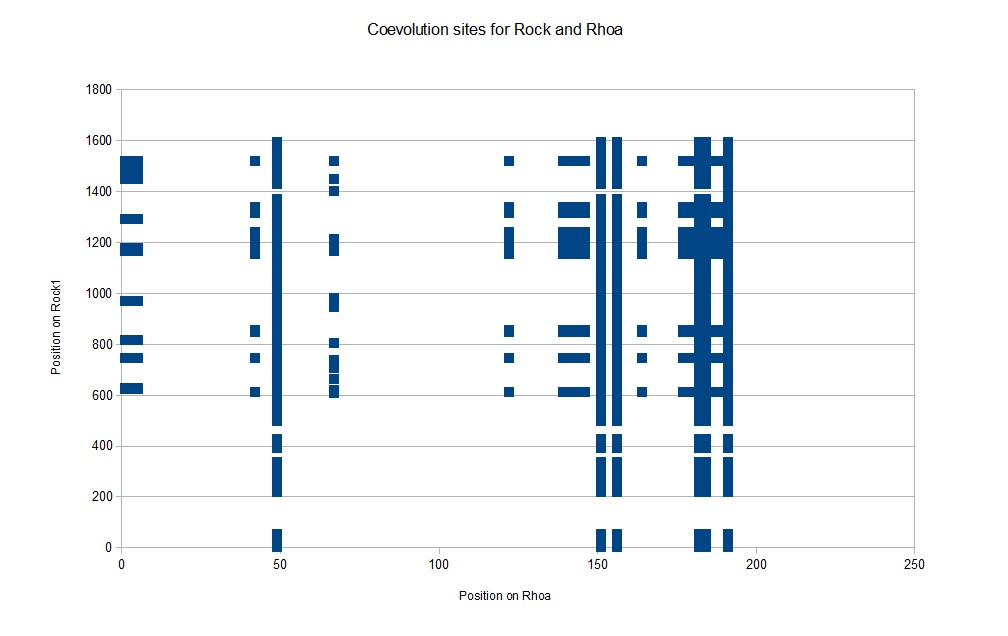
\includegraphics[width=6.5in,height=4.1in]{pos.png}
Graph 1 Positions of amino acids exhibiting covariance for the proteins Rock1 and RhoA, as determined by our program.  On Rhoa, amino acid 49 represents a solvent exposed amino acid.  Many of the other co-varying sites, such as the block of 10 amino acids around 190, are present in the interaction site between the two proteins.\\

\newpage

\begin{center}
\textbf{Reflection}
\end{center}

%This project exposed the entire group to new material. Overall, our group learned that interprotein coevolution analysis is very difficult which is why very few have succeeded in creating a program that provides accurate information. In hindsight, we would have approached the problem differently from the start by dividing the tasks evenly and with more thought into what we wanted to accomplish. The BLAST search should have been done first. Right now, our program is designed to compare two entirely different proteins but if we had more time, we would modify the program to observe individual regions and how they coevolve with another region on a different protein.  If we had more time, paralogs would be taken into because the program now does not consider the fact that it could be filtering for a version that is similar but not the actual version that binds to the substrate protein anymore.

For everyone except for Kyle the idea that one could compare the
changes in the amino acids in a protein to get an idea of how much
they interacted was completely new. As such all of us were exposed to
a new way of thinking that we had never experienced before. Although
Kyle was already familiar with the Biological side of the project he
got to learn a great deal about what the Computer Science side is
capable of. Although our results are inconclusive at best and
downright useless at the worst we all believe that it was a good
project and we learned a tremendous amount. \\

In retrospect it would have been good to get the BLAST search results
sooner in the project since they were necessary to do any actual
analysis of the proteins. Since we didn't have these as early as would
have been desirable we had no idea what our test was actually going to
do until it was too late to do more analysis and come up with a better
protein scoring system. That being said we likely would not have a
working system even if we had started with the BLAST results. \\

As such there are several things that we would have liked to do in the
next month or so of the project. First it would probably be a good
idea to do a bit of house cleaning on the code since it got a little
messy while we were tweaking all of the settings. \\

Second it would have been really useful to try to apply the results of
intra-protein analysis to inter-protein analysis. It is our belief
that by using the intra-protein analysis it would be possible to
eliminate a much larger portion of the "false positive" mutations that
look like coevolution events but are instead just random chance. Our
results are currently far to crude to draw any sort of conclusions
from them. \\

It would also be nice to spend some time improving the pipeline with
an auto-grading system that would report whether or not our changes
improved the scoring system or had no effect. This would allow us to
make changes more quickly and would be an easy that could easily be
finished within a month. \\

Furthermore it would be interesting to run some docking simulations to
see if any of the results that could possibly be newly discovered
interactions actually hold any weight when simulated. If so it would
be even more intriguing to actually carry out an experiment to confirm
the interaction.
\end{document}
